\documentclass[lecture.tex]{subfiles}

\begin{document}

\exercice{}
%\video{https://youtu.be/blablabla}
\enonce{rdm-0015}{Flexion d’une poutre (section rectangulaire)}


\begin{center}
  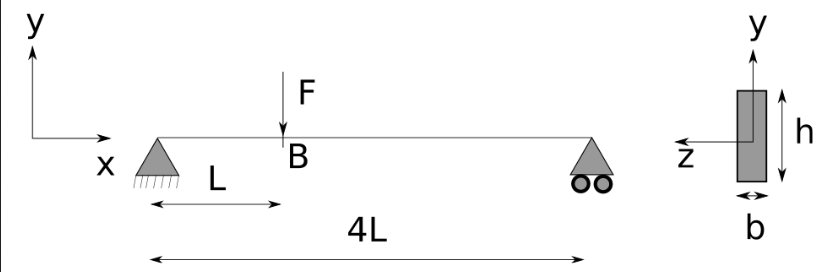
\includegraphics[scale=0.5]{exo-flexion-poutre.png}
\end{center}

\begin{enumerate}
  \item Identifier les inconnues de liaison
  \item Trouver les efforts internes de la poutre.
  \item Tracer les graphes des efforts internes.
  \item Trouver le fléchissement ($v(x)$ et $\theta(x)$) de la poutre en fonction de $x$.
\end{enumerate}

\finenonce{rdm-0015}
\finexercice


\end{document}
